\chapter{基于信息通信模型的隐私度量模型}
\label{chap:entropy-metric-model}

\textit{ }

\textit{本章针对目前隐私量化缺乏对隐私定义、隐私分析、隐私保护等统一的量化框架的问题,基于Shannon信息论的通信框架提出了几种隐私保护信息熵模型。在所提出的度量模型中,将信息拥有者假设为发送方,隐私谋取者假设为接收方,隐私的泄露渠道假设为通信信道;基于该假设,分别引入信息熵、平均互信息量、条件熵及条件互信息等来分别描述隐私保护系统信息源的隐私度量、隐私泄露度量、含背景知识的隐私度量及泄露度量;以此为基础,进一步提出了隐私保护方法的强度和敌手攻击能力的量化,为隐私泄露的量化风险评估提供了一种支撑;最后,针对位置隐私保护的应用场景,给出了具体的信息熵模型及隐私保护机制和攻击能力的度量及分析。本章成果已发表在《软件学报》。}

\section{概述}

隐私保护的研究起步较早,但近年来突然受到产业界和学术界的广泛关注是因为大数据的不期而至,隐私保护成为大数据应用的主要瓶颈,移动网络、社交网络、基于位置服务等新型应用服务的推进,隐私问题更加突出。目前关于隐私保护有两个方向值得关注:一是研究隐私保护算法以更加有效的方式保护隐私;二是通过研究隐私泄露风险分析与评估。隐私保护算法目前主要集中在匿名方法,包括~$k$~匿名、~$l$~多样性匿名和~$t$~接近匿名及其衍生的方法。隐私度量最早起源于相关匿名算法~\cite{sweeney2002k}, 在匿名隐私保护算法的研究过程中,不时有学者关注隐私量化问题,尤其是在定位服务领域,位置匿名及轨迹匿名算法上已有不少隐私度量的相关研究\cite{shokri2011quantifying,olteanu2017quantifying},因此对于隐私保护算法来说,隐私度量仍需进一步深入研究。然而就目前来说,隐私泄露涉及因素众多,设计有效的隐私保护算法仍然是挑战性问题,但政府及企业数据开放共享中迫切的隐私保护需求,促使我们不得不在可用性与隐私泄露之间寻求一种平衡,要解决这个问题,隐私风险分析及评估不失为一种方法。风险分析依然涉及到隐私量化问题,也就是说量化风险评估不失为隐私保护一种可行的解决方案,量化隐私风险必然也涉及隐私度量问题。从这些分析来看,隐私度量的研究具有十分重要的理论意义和应用价值。

信息熵作为信息度量的有效工具,在通信领域已展现出其重要的贡献。隐私作为一种信息,自然可以考虑用熵来量化,为此,不少学者或多或少进行了探索,比如事件熵、匿名集合熵、条件熵等\cite{serjantov2002towards,diaz2002towards,wagner2018technical},但其研究还较为零散,更多是针对某一具体领域,如位置隐私保护领域,目前尚未形成统一的模型及体系,其应用范围也受到限制,特别是隐私是具有时空性的,与人的主观感受也有关系,不同的人对同一隐私的认同可能不同。 鉴于以上分析,本章旨在参考Shannon信息论的通信框架\cite{stone2018information},提出几种隐私保护信息熵模型,包括隐私保护基本信息熵模型、含敌手攻击的隐私保护信息熵模型、带主观感受的信息熵模型和多隐私信源的隐私保护信息熵模型。在这些模型中,将信息拥有者假设为发送方,隐私谋取者假设为接收方,隐私的泄露渠道假设为通信信道;基于这样的假设,分别引入信息熵、平均互信息量、条件熵及条件互信息等来分别描述隐私保护系统信息源的隐私度量、隐私泄露度量、含背景知识的隐私度量及泄露度量;以此为基础,进一步提出了隐私保护方法的强度和敌手攻击能力的量化测评,力图为隐私泄露的量化风险评估提供一种理论支持。


\section{相关工作}\label{related work}

信息熵理论是Shannon于1948年提出的,解决了信息的量化和通信的理论基础。较早将信息熵考虑到隐私度量的研究是Diaz等\cite{diaz2002towards}和Serjantov等\cite{serjantov2002towards},他们提出了用信息熵来度量匿名通信系统的匿名性,在假定攻击者的目的是确定消息的发送者(或接收者)的真实身份的情况下,系统中每个用户都以一定的概率被猜测为消息的真实发送者(或接收者),将攻击者猜测某用户是真实发送者(或接收者)看成一个随机变量$X$,用信息熵$H(X)=-\sum p(x)\log p(x)$来量化的随机变量的不确定性可表征为系统的隐私水平。随后,有不少学者将信息熵应用于某些具体领域的隐私度量,如位置服务、社交网络和数据挖掘等领域,对于不同的方案\cite{serjantov2002towards,shokri2011quantifying,wang2012location},其随机变量的概率表现形式和对熵的处理方式不同。在位置服务领域,2007年,Hoh等\cite{hoh2007preserving}提出了基于信息熵的隐私度量方法度量轨迹跟踪的不确定度,其中随机变量的概率表现为每个位置实例包含在当前跟踪车辆轨迹的概率。2009年,Ma等\cite{ma2009measuring}提出在V2X车联网系统中信息熵的隐私度量方法,其中随机变量的概率表现为每个位置信息关联到某特定用户的概率,该方法还考虑了随机变量的概率随着时间的变化而更新的情况,也即攻击者的累积信息对系统隐私的影响。同年,林欣等\cite{lin2009lbs}针对LBS中的连续查询问题,提出一种连续查询攻击算法,指出匿名集的势不再适合作为查询该算法匿名性的度量,并提出了基于信息熵的度量方法,其中随机变量的概率表现为每个用户$u_{i}$是查询$q$的真正发出者的概率,信息熵计算为$H(q)$,用$AD(q)=2^{H(q)}$度量为系统的隐私水平。2011年,Shokri等\cite{shokri2011quantifying}将位置隐私的度量准则分为精确性、确定性和正确性,精确性度量为攻击者猜测事件的置信区间,确定性度量为攻击者猜测的不确定性,正确性度量为攻击者出错的概率,其中精确性的度量是基于信息熵的度量方法,随机变量的概率表现为每个观测事件是真实事件的概率。2012年,Chen等\cite{chen2012measuring}针对LBS查询隐私进行度量,随机变量的概率表现为攻击者在无背景知识和有背景知识两种情况下的判断用户$u_{i}$是查询$q$的真实发出者的条件概率,并利用互信息$I(U|q;<r,t,q>)=H(U|q)-H(U|<r,t,q>)$度量系统的隐私水平。同年,王彩梅\cite{wang2012location}等针对LBS中的轨迹隐私保护方法Silent Cascade提出基于信息熵的隐私度量方法,随机变量的概率表现为某用户的每条可能轨迹的概率,特定用户的熵计算为$H(u_{i})$,并用标准熵$D(u_{i})=H(u_{i})/H_{max}(u_{i})$度量为系统的隐私水平。2014年,文献\cite{niu2014achieving,olteanu2017quantifying}均采用了信息熵度量了LBS系统的隐私水平。

在社交网络领域,2010年,Ngoc等\cite{ngoc2010new}针对社交网络隐私泄露的情况,提出了基于信息熵的隐私度量方法,以帮助用户判断所发布信息的隐私水平,其随机变量的概率表现为事件\textit{X}的取值\textit{x}的概率。2012年,Yang等\cite{yang2012stalking}总结了社交网络中的风险,并利用信息熵和互信息度量的系统的隐私水平。

此外,信息熵在其它领域的隐私度量中也有所涉及,文献\cite{agrawal2001design,zhan2007quantifying}研究了信息熵用于数据挖掘领域的隐私度量,文献\cite{edman2007combinatorial}研究了信息熵用于匿名系统领域的隐私度量,文献\cite{wagner2017evaluating}研究了信息熵基因序列隐私的隐私度量,Wagner等\cite{wagner2018technical}对当前存在的隐私度量方法进行了综述,根据度量系统的输出将隐私度量方法分成八类,其中不确定度的分类中是根据信息熵来度量的。

综上可知,目前存在的基于信息熵进行隐私度量的理论体系较为零散,缺乏统一的模型基础。针对上述问题,本章试图将隐私保护系统看作一个通信模型,力图探讨较为通用的隐私度量信息熵模型,解决隐私度量的一些基本概念和基础体系。

\section{隐私保护信息熵模型}\label{sec:Entropy model of privacy protection information}

本章的出发点是将信息拥有者假设为发送方,隐私谋取者(敌手)假设为接收方,隐私的泄露渠道假设为通信信道。

发送方拥有的一个信息集称为隐私信源,用随机变量$X$表示,$X$是由所有的离散基本泄露事件的隐私消息构成的隐私消息空间,即$\left \{ x_{1},x_{2},...,x_{i},...,x_{n} \right \}$,其中$x_{i}(i=1,2,...,n)$为基本泄露事件的隐私消息;接收方获取的信息集称为隐私信宿,用随机变量$Y$表示,$Y$是由敌手获取的所有基本隐私消息构成,即$\left \{y_{1},y_{2},...,y_{j},...,y_{m} \right \}$,其中$y_{j}(j=1,2,...,m)$为敌手获取的某个隐私消息。相应的,某一种具体的隐私保护算法可以看作是对隐私消息进行转换、编码的方法,它能够对隐私消息进行干扰进而实现对隐私信息的保护,其中隐私保护算法的全体构成隐私保护机制空间,称为隐私保护机制源。敌手在一定背景知识下对隐私信息的挖掘与分析手段称为隐私攻击,所有隐私方法的的全体称为隐私攻击空间。

以此假设为基础,本节将基于Shannon信息论的通信框架\cite{stone2018information}提出几种隐私保护信息熵模型,包括:隐私保护基本信息熵模型、含敌手攻击的隐私保护信息熵模型、带主观感受的信息熵模型和多隐私信源的隐私保护信息熵模型。通过引入隐私信息熵、平均互信息量、条件熵及条件互信息等来分别描述隐私保护系统信息源的隐私度量、隐私泄露度量、含背景知识的隐私度量及泄露度量。

\subsection{隐私保护基本信息熵模型}

这里我们首先假设敌手无任何隐私攻击能力,敌手仅通过信道观测到隐私信息,并只考虑离散单隐私信源的情形。模型定义为
\begin{figure}[htbp]
	\centering
	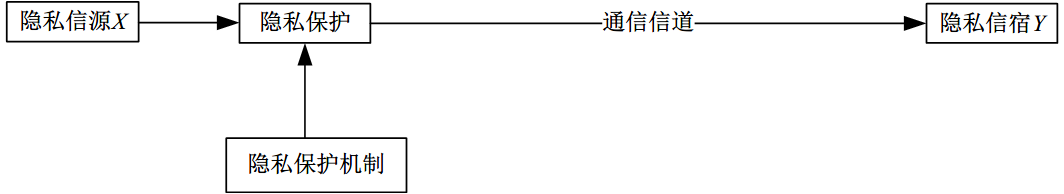
\includegraphics[width = 0.95\linewidth]{./figures/Communication-Model-for-Privacy.png}
	\caption{单隐私信源隐私保护通信模型}
	\label{fig:communication-model-privacy}
\end{figure}

图\ref{fig:communication-model-privacy}中,设单隐私信源$X$的数学模型可以表示为
\begin{equation}
\begin{pmatrix}
X\\ 
P(X)
\end{pmatrix}=\begin{pmatrix}
x_{1} & x_{2} & \cdots  & x_{i} & \cdots  & x_{n}\\ 
p(x_{1})& p(x_{2}) & \cdots & p(x_{i}) & \cdots & p(x_{n})
\end{pmatrix}
\end{equation}
其中$0\leqslant p(x_{i})\leqslant1$,$\sum_{i=1}^{n}p(x_{i})=1$。同理,隐私信宿$Y$的数学模型可表示为
\begin{equation}
\label{eq:single-information-source}
\begin{pmatrix}
Y\\ 
P(Y)
\end{pmatrix}=\begin{pmatrix}
y_{1} & y_{2} & \cdots  & y_{i} & \cdots  & y_{m}\\ 
p(y_{1})& p(y_{2}) & \cdots & p(y_{i}) & \cdots & p(y_{m})
\end{pmatrix}
\end{equation}

针对该模型,定义\textbf{隐私信源熵}$H(X)$为
\begin{equation}
H(X)=-\sum_{i=1}^{n}p(x_{i})\log_{2}p(x_{i})
\end{equation}
其中,$H(X)$用于刻画隐私信源的平均隐私信息量,也是隐私信源的隐私不确定程度,$H(X)$越大,隐私泄露就可能越小,从而它亦可以用于衡量隐私的保护程度,在没有外部条件影响时,该值是一个确定的值。

当隐私信宿$Y$在获取隐私信息条件下,关于隐私信源的不确定程度,可以引入\textbf{隐私条件熵}$H(X/Y)$刻画,其定义为
\begin{equation}
H(X/Y)=-\sum_{j=1}^{m}\sum_{i=1}^{n}p(x_{i}y_{j})\log_{2}p(x_{i}/y_{j})
\end{equation}

该条件熵表示隐私信宿在收到$Y$后,隐私信源$X$仍然存在的不确定程度,该不确定程度是隐私泄露信道的干扰(隐私保护)造成的,即敌手在长期观测隐私信源过程中,由于隐私保护机制的保护下,敌手对隐私信源仍然存在一定的不确定。

易证上述的隐私信息熵是满足Shannon信源熵的基本性质。即具有非负性、对称性、扩展性、确定性、可加性、极值性、上凸性等,并满足极大离散熵定理,在此不再赘述。

下面引入\textbf{平均隐私互信息量}$I(X,Y)$来刻画信道上隐私泄露程度,定义为
\begin{equation}
I(X;Y)=\sum_{i=1}^{n}\sum_{j=1}^{m}p(x_{i}y_{j})\log_{2}\frac{p(x_{i}/y_{j})}{p(x_{i})}
\end{equation}
其中,$I(X;Y)$表示了隐私信源$X$和隐私信宿$Y$之间交互的平均信息量,即在信道上传送的隐私信息量,它正好可以刻画隐私的整体泄露程度,从而可用于度量隐私的泄露。

\subsection{含敌手攻击的隐私保护信息熵模型}\label{subsec:privacy-preserving-attack}

上节提出的隐私保护基本信息熵模型客观上描述了无敌手攻击或敌手无攻击能力情况下的隐私度量问题。在实际系统中往往存在着隐私攻攻击分析分析,敌手可以在一定的背景知识下进行攻击分析,模型定义为
\begin{figure}[htbp]
	\centering
	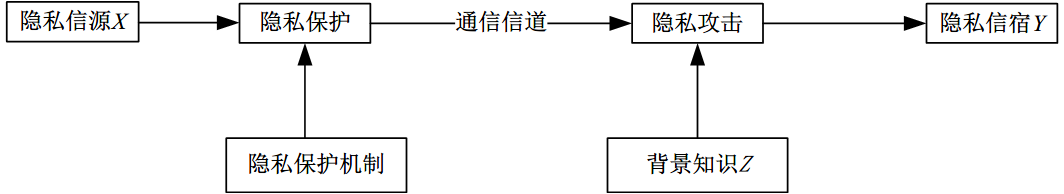
\includegraphics[width = 0.95\linewidth]{./figures/Communication-Model-for-Privacy-of-Single.png}
	\caption{单隐私信源且敌手具备知识背景的隐私保护通信模型}
	\label{fig:Communication-Model-for-Privacy-of-Single}
\end{figure}

在图\ref{fig:Communication-Model-for-Privacy-of-Single}所示模型中,表示背景知识空间,其数学模型亦可定义为
\begin{equation}
\begin{split}
&\begin{pmatrix}
Y\\ 
P(Y)
\end{pmatrix}=\begin{pmatrix}
y_{1} & y_{2} & \cdots  & y_{i} & \cdots  & y_{m}\\ 
p(y_{1})& p(y_{2}) & \cdots & p(y_{i}) & \cdots & p(y_{m})
\end{pmatrix} \\
&0 \leqslant p(z_{k})\leqslant 1,\sum_{k=1}^{l}p(z_{k})=1(k=1,2,...,l)
\end{split}
\end{equation}

攻击者可以利用背景知识$Z$加强对隐私进行攻击,对于攻击者来说,可以联合隐私信宿消息$Y$和背景知识$Z$进行隐私分析攻击,引入\textbf{攻击条件熵}
\begin{equation}
H(X/YZ)=\sum_{i=1}^{n}\sum_{j=1}^{m}\sum_{k=1}^{l}p(x_{i}y_{j}z_{k})\log_{2}p(x_{i}/y_{j}z_{k})
\end{equation}
\begin{equation*}
I(X;Y/Z)
\end{equation*}

$H(X/YZ)$反映了攻击者在获得隐私信宿消息$Y$和背景知识$Z$后,关于$X$仍然存在的不确定度,它实际了可以作为在具有攻击分析的情况下隐私信息的不确定度,亦可以作为隐私保护强度的度量。进一步定义\textbf{隐私攻击平均互信息}$I(X;Y/Z)$
\begin{equation}
I(X;Y/Z)=\sum_{i=1}^{n}\sum_{j=1}^{m}\sum_{k=1}^{l}p(x_{i}y_{j}z_{k})\log_{2}\frac{p(x_{i}z_{k}/y_{j})}{p(x_{i}/z_{k})p(y_{j}/z_{k})}
\end{equation}

上述公式反映了得到$Z$的条件下,$X$和$Y$之间的平均互信息量,即接收方获得的隐私信息量,即可以刻画具有背景知识攻击下的隐私泄程度。

\subsection{带主观感受的信息熵模型}

信息源发生的隐私事件所泄露的隐私信息是客观存在的,但通常对隐私信息是带有主观感受的,不同的隐私信息的重要程度不同或价值不同。本节将权重引入前两节的信息熵模型中,对含有主观感受的隐私信源的隐私信息进行度量。

\textbf{(1) 带主观感受的隐私保护信息熵模型}

针对图\ref{fig:communication-model-privacy}所述通信模型。隐私信源发出的消息$x_{i}(i=1,2,...,n)$,确定一个非负实数作为该消息的重要程度权值,不同的消息,权值越大,重要程度越大。可对该隐私信源建立权值空间
\begin{equation}
\centering
\begin{split}
&\begin{pmatrix}
X\\ 
W(X)
\end{pmatrix}=\begin{pmatrix}
x_{1} & x_{2} & \cdots  & x_{i} & \cdots  & x_{n}\\ 
w(x_{1})& w(x_{2}) & \cdots & w(x_{i}) & \cdots & w(x_{n})
\end{pmatrix} \\
&w_{i}\geqslant 0(i=1,2,...,n)
\end{split}
\end{equation}

定义\textbf{隐私加权信源熵}$H_{w}(X)$对隐私信源的隐私信息加权平均隐私信息$w_{i}(i=1,2,...,n)$量进行度量,并刻画了隐私信源对隐私消息的主观感受影响信源的隐私信息量。在相对稳定的时间段内,隐私信源对隐私消息的主观感受或偏好一旦固定,隐私加权信源熵是一个确定的值。

\begin{equation}
H_{w}(X)=-\sum_{i=1}^{n}w_{i}p(x_{i})\log_{2}p(x_{i})
\end{equation}

隐私信源加权熵显然有以下性质。
\begin{itemize}
	\item 非负性。无论一个隐私事件的重要程度如何,隐私信源一旦发生了一个隐私事件,其总能提供一定关于隐私信息的信息量。
	\item 连续性。隐私信源发生的隐私事件的概率发生微小的变动,形成另一个隐私信源,变化前后的两个隐私信源的加权熵是连续的。该特性对于刻画因时间变化,隐私信源的特性变化是非常有效的。如在某一段时间内,一个人的生活规律是固定的,导致其能够泄露个人隐私的行为模式的概率分布是相对固定的,但随时间的推移,此人的生活规律会连续性的发生微小的变化,进而能够泄露其隐私的行为模式概率分布也发生了微小的变动。但行为发生变化前后关于行为总体的加权熵是连续的。
\end{itemize}

除此之外,隐私信源加权熵还有对称性,均匀性等不同性质,并在隐私保护系统中有相应的实际意义。仅考虑隐私信源对隐私消息的主观感受,定义\textbf{隐私加权条件熵}$H_{w}(X/Y)$刻画隐私谋取者对信息拥有者的隐私信息平均不确定程度。
\begin{equation}
H_{w}(X/Y)=-\sum_{i=1}^{n}w_{i}\sum_{j=1}^{m}p(x_{i}y_{j})\log_{2}p(x_{i}/y_{j})
\end{equation}

同样, 仅考虑隐私信源对隐私消息的主观感受,定义\textbf{隐私加权平均互信息}$I_{w}(X;Y)$刻画信息拥有者发生了隐私事件之后,在隐私保护机制的保护下,隐私谋取者观测到的隐私事件后接收到关于信息拥有者的隐私信息量。
\begin{equation}
I_{w}(X;Y)=-\sum_{i=1}^{n}w_{i}\sum_{j=1}^{m}p(x_{i}y_{j})\log_{2}\frac{p(x_{i}/y_{j})}{p(x_{i})}
\end{equation}

这里,隐私加权条件熵和隐私加权平均互信息仅考虑了隐私信源对隐私消息的主观感受和偏好,在实际系统中,不仅仅是信息拥有者对自身的隐私信息有不同的主观感受,隐私谋取者对获取到的隐私信息也有不同的主观感受和偏好。故可以进一步探讨通信模型中隐私信宿对隐私消息的主观感受并赋予权值,甚至建立刻画隐私信源和隐私信宿双方偏好的权值矩阵,定义更加符合实际的隐私加权条件熵和隐私加权平均互信息。

\textbf{(2) 带主观感受并含敌手攻击的隐私保护信息熵模型}

在本模型中,仍然仅考虑隐私拥有者对其隐私信息的主观感受和偏好。故隐私信源$X$的\textbf{隐私加权信源熵}$H_{w}(X)$定义如公式。同时定义\textbf{加权攻击条件熵}$H_{w}(X/YZ)$隐私信宿在具备攻击能力后对在主观感受的隐私信源隐私信息的平均不确定程度,可以作为隐私保护在敌手攻击下的保护强度度量。
\begin{equation}
H_{w}(X/YZ)=-\sum_{i=1}^{n}w_{i}\sum_{j=1}^{m}\sum_{k=1}^{l}p(x_{i}y_{j}z_{k})\log_{2}p(x_{i}/y_{j}z_{k})
\end{equation}

在此基础上定义\textbf{隐私攻击加权平均互信息}$I(X;Y/Z)$表示在得到$Z$的条件下,隐私信宿接收到的隐私信息量,具体刻画在具有背景知识条件下隐私泄露的量。
\begin{equation}
I(X;Y/Z)=\sum_{i=1}^{n}w_{i}\sum_{j=1}^{m}\sum_{k=1}^{l}p(x_{i}y_{j}{x}'_{k})\log_{2}\frac{p(x_{i}z_{k}/y_{j})}{p(x_{i}/z_{k})p(y_{j}/z_{k})}
\end{equation}

\subsection{多隐私信源的隐私保护信息熵模型}

客观上,系统中的信息拥有者是多个的,其带有隐私信息的隐私事件通过隐私保护机制进行保护。故可建立多隐私信源的隐私保护通信模型,对相互关联的多个信源的隐私信息的保护和攻击进行度量。 如图\ref{fig:Communication-Model-for-Privacy-of-Multi-Source}所示的无隐私攻击的多隐私信源隐私保护通信模型和图\ref{fig:Communication-Model-for-Privacy-of-Multi-Source-attacks}所示的带隐私攻击的多隐私信源隐私保护通信模型。

\textbf{(1) 多隐私信源的隐私保护信息熵模型}

\begin{figure}[htbp]
	\centering
	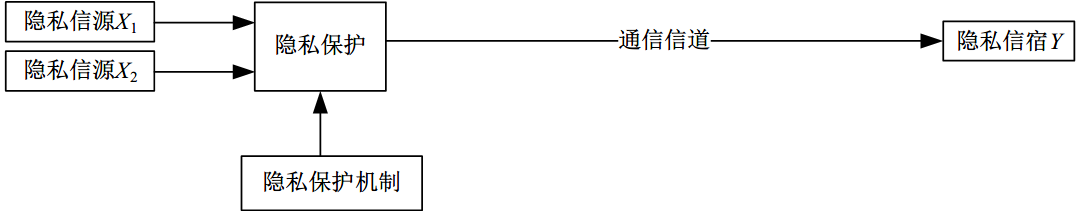
\includegraphics[width = 0.95\linewidth]{./figures/Communication-Model-for-Privacy-of-Multi-Source.png}
	\caption{无隐私攻击的多隐私信源隐私保护通信模型}
	\label{fig:Communication-Model-for-Privacy-of-Multi-Source}
\end{figure}

在图\ref{fig:Communication-Model-for-Privacy-of-Multi-Source}所示的通信模型中,隐私信源$X_{1}$和隐私信源$X_{2}$共同构成隐私信源$X$,其数学模型为
\begin{equation}
\begin{split}
&\begin{pmatrix}
X_{1}\\ 
P(X_{1})
\end{pmatrix}=\begin{pmatrix}
x_{11} & x_{12} & \cdots  & x_{1i_{1}} & \cdots  & x_{1n_{1}}\\ 
p(x_{11})& p(x_{12}) & \cdots & p(x_{1i_{1}}) & \cdots & p(x_{1n_{1}})
\end{pmatrix} \\
&0\leqslant p(x_{i_{1}})\leqslant 1,\sum_{i_{1}=1}^{n_{1}}p(x_{i_{1}})=1(i_{1}=1,2,...,n_{1})
\end{split}
\end{equation}
\begin{equation}
\begin{split}
&\begin{pmatrix}
X_{2}\\ 
P(X_{2})
\end{pmatrix}=\begin{pmatrix}
x_{21} & x_{22} & \cdots  & x_{2i_{2}} & \cdots  & x_{2n_{2}}\\ 
p(x_{21})& p(x_{22}) & \cdots & p(x_{2i_{2}}) & \cdots & p(x_{2n_{2}})
\end{pmatrix} \\
&0\leqslant p(x_{i_{2}})\leqslant 1,\sum_{i_{2}=1}^{n_{2}}p(x_{i_{2}})=1(i_{2}=1,2,...,n_{2})
\end{split}
\end{equation}

隐私信宿$Y$的数学模型如公式\ref{eq:single-information-source}所述,定义\textbf{多源联合隐私信源熵}$H(X_{1}X_{2})$,该信源熵刻画的多个带关联的隐私拥有者的隐私信息的量。
\begin{equation}
H(X_{1}X_{2}) = -\sum_{i_{1}=1}^{n_{1}}\sum_{i_{2}=1}^{n_{2}}p(x_{i_{1}}x_{i_{2}})\log_{2}p(x_{i_{1}}x_{i_{2}})=H(X_{1})+H(X_{2}/X_{1})
\end{equation}
已知隐私信宿$Y$条件下对隐私信源$X$的\textbf{多源联合隐私条件熵}为$H(X/Y)=H(X_{1}X_{2}/Y)=H(X_{1}X_{2}Y)-H(Y)$。该定义刻画的是多个带关联的信息拥有者发生的隐私事件在隐私保护后,隐私信息获取者对被保护的隐私事件进行观测后其对各信息拥有者的隐私信息的平均不确定程度。

同时,定义\textbf{多源联合平均互信息}$I(X_{1}X_{2};Y)$刻画多个带关联的信息拥有者发生的隐私事件在隐私保护后,隐私信息谋取者通过观测被保护隐私事件后获取的各信息拥有者的隐私信息量。
\begin{equation}
I(X_{1}X_{2};Y)=\sum_{i_{1}=1}^{n_{1}}\sum_{i_{2}=1}^{n_{2}}\sum_{j=1}^{m}p(x_{i_{1}}x_{i_{2}}y_{j})\log_{2}\frac{p(x_{i_{1}}x_{i_{2}}/y_{j})}{p(x_{i_{1}}x_{i_{2}})}
\end{equation}

\textbf{(2) 多隐私信源带隐私攻击的隐私保护信息熵模型}

在\ref{subsec:privacy-preserving-attack}节所提带隐私攻击的隐私保护信息熵模型基础上,引入多个带关联的信息拥有者,构成新的关联的多隐私信源,并可进一步构建多隐私信源带隐私攻击的隐私保护信息熵模型,其通信模型如图\ref{fig:Communication-Model-for-Privacy-of-Multi-Source-attacks}所示。

\begin{figure}[htbp]
	\centering
	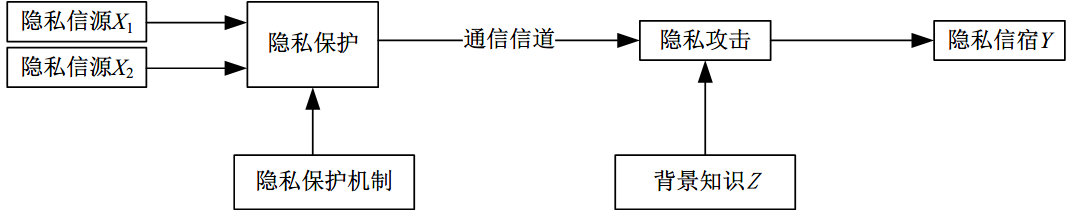
\includegraphics[width = 0.95\linewidth]{./figures/Communication-Model-for-Privacy-of-Multi-Source-attacks.png}
	\caption{带隐私攻击的多隐私信源隐私保护通信模型}
	\label{fig:Communication-Model-for-Privacy-of-Multi-Source-attacks}
\end{figure}

图\ref{fig:Communication-Model-for-Privacy-of-Multi-Source-attacks}所述通信模型的信源数学模型如公式和,隐私信宿$Y$的数学模型如公式公式\ref{eq:single-information-source}所述。该模型下的\textbf{多源联合信源熵}$H(X)=H(X_{1}X_{2})$,\textbf{多源联合隐私攻击条件熵}$H(X_{1}X_{2}/YZ)$和\textbf{多源联合隐私攻击条件平均互信息}$I(X_{1}X_{2};Y/Z)$,其中多源联合隐私攻击条件熵表示的在已知背景知识攻击下接收者对联合隐私信源的隐私信息的不确定度; 多源联合隐私攻击条件平均互信息表示在已知背景知识攻击下接收者收到的联合隐私信源隐私消息所含的隐私信息量。

\begin{equation}
\begin{split}
&H(X_{1}X_{2}/YZ)=H(X_{1}X_{2}YZ)-H(YZ)\\
&I(X_{1}X_{2};Y/Z)=H(X_{1}X_{2})-H(X_{1}X_{2}Y/Z)
\end{split}
\end{equation}

\section{隐私度量及其对隐私保护机制和隐私攻击手段的评价}\label{Privacy measures}
应用信息熵和平均互信息对隐私信息进行度量,并以此为基础对隐私保护机制的有效性建立评价方法,同时对隐私保护机制对隐私攻击手段的抗攻击能力建立测评方法。

\subsection{隐私度量方法}
针对隐私保护基本信息熵模型,直观地可以用条件熵和互信息在该模型下,对隐私保护机制保护下的隐私进行度量。

针对某一隐私信源,可以应用不同的隐私保护机制对隐私信源发送的隐私消息进行保护,调整能够让隐私信宿接收到的消息的概率分布,改变信宿的熵。以隐私信宿的视角,在接收到被保护后的隐私消息,仍然对隐私信源的隐私信息有一个平均不确定程度,这个程度应用隐私条件熵$H(X/Y)$做量化。记应用某一具体隐私保护机制$P_{i}$的对隐私信源$X$发送的消息件进行保护后的隐私条件熵为$H_{P_{i}}(X/Y)$,则期望该条件熵尽可能大。

平均互信息刻画的是经过信息传输后,信宿所接收到的平均信息量。隐私平均互信息$I(X;Y)$表示的是隐私信宿$X$在隐私保护机制的保护下隐私消息被隐私信宿$Y$所接收到的平均隐私信息量。记应用某一具体隐私保护机制$P_{i}$的对隐私信源$X$发送的消息件进行保护后,隐私信宿$Y$接收到的隐私信息为$I_{P_{i}}(X;Y)$,则期望该隐私互信息能尽可能小。

\begin{property}
应用隐私条件熵和隐私互信息进行隐私度量,具有一致性。
\end{property}
\begin{proof}
	由公式知
	\begin{equation}
	\begin{split}
	I(X;Y)&=\sum_{i=1}^{n}\sum_{j=1}^{m}p(x_{i}y_{j})\log_{2}\frac{p(x_{i}/y_{j})}{p(x_{i})}\\
	&=\sum_{i=1}^{n}\sum_{j=1}^{m}p(x_{i}y_{j})\log_{2}\frac{1}{p(x_{i})}-\sum_{i=1}^{n}\sum_{j=1}^{m}p(x_{i}y_{j})\log_{2}\frac{1}{p(x_{i}/y_{j})}\\
	&=\sum_{i=1}^{n}p(x_{i})\log_{2}\frac{1}{p(x_{i})}-\sum_{i=1}^{n}\sum_{j=1}^{m}p(x_{i}y_{j})\log_{2}\frac{1}{p(x_{i}/y_{j})}\\
	&=H(X)-H(X/Y)
	\end{split}
	\end{equation}
	
	故有$I(X;Y)=H(X)-H(X/Y)$,易知隐私信源熵是一个确定的值,隐私条件熵越大,则隐私平均互信息越小。
\end{proof}


针对含敌手攻击的隐私保护信息熵模型,隐私度量主要是对隐私信宿本身含有的隐私信息量;敌手在背景知识条件下对发送者的隐私信息进行攻击时,发送者隐私信息的保护强度;以及在敌手攻击下,信息拥有者所泄露的隐私信息量。

隐私信宿本身含有的隐私信息量可用隐私信源熵$H(X)$的大小进行度量,其表示信息拥有者隐私信息的固有量的多少,一旦隐私信宿确定,则此隐私信宿所拥有的隐私信息量就是一个确定的值。

系统隐私度量综合考虑经过隐私保护和隐私攻击后,在一定背景知识条件下,隐私谋取者对信息拥有者的隐私信息的不确定程度$H(X/YZ)$;以及隐私谋取者观测信息拥有者发生的隐私事件所包含的隐私信息量$I(X;Y/Z)$。系统中应用隐私保护机制$P_{i}$进行隐私保护和隐私攻击$A_{r}$进行隐私攻击,则分别记$H_{P_{i},A_{r}}(X/YZ)$和$I_{P_{i},A_{r}}(X;Y/Z)$作为系统在抵抗攻击$A_{y}$下采用$P_{i}$的隐私信息泄露的隐私度量值。$H_{w}(X)H(X_{1}X_{2})$

\subsection{隐私保护机制及隐私攻击评价}
\textbf{(1)隐私保护基本信息熵模型下的隐私保护机制评价}

应用隐私保护机制对信息拥有者的隐私信息进行保护,$H_{w}(X/Y)$目标是使隐私信息尽可能少的被隐私谋取者所获得,即期望通过某种隐私保护机制,使得隐私谋取者得到的信息量$I(X;Y)$尽可能小,最好是0。
\begin{definition}
	\label{def:perfec-privacy-preserving}
	若在某种隐私保护机制的保护下,隐私平均互信息$I(X;Y)=0$(隐私信宿从隐私信源接收到的隐私信息量为0),则称该隐私保护机制对此信源是\textbf{完全隐私保护}的。
\end{definition}

\begin{definition}
\label{def:partial-ordering}	
	 对同一隐私信源$X$分别应用隐私保护机制$P_{i}$和$P_{j}$对隐私消息进行保护,若\\$H_{P_{i}}(X/Y)<H_{P_{j}}(X/Y)$(或$I_{P_{i}}(X;Y)>I_{P_{j}}(X;Y)$),则称隐私保护机制$P_{j}$比隐私保护机制$P_{i}$\textbf{隐私保护有效性好},简记偏序关系$P_{i}\prec P_{j}$。若$H_{P_{i}}(X/Y)=H_{P_{j}}(X/Y)$(或$I_{P_{i}}(X;Y)=I_{P_{j}}(X;Y)$),则称隐私保护机制$P_{i}$与隐私保护机制$P_{j}$\textbf{隐私保护有效性相等},简记等价关系$P_{i}\cong P_{j}$
\end{definition}

\begin{theorem}
	\label{thm:distance-properties}
	设隐私保护机制有效性偏序关系与等价关系如定义\ref{def:partial-ordering}所定义,则偏序关系具有可传递性,等价关系具有自反性,可传递性,对称性。
\end{theorem}

\begin{proof}
	若有$P_{i}\prec P_{j},P_{j}\prec P_{k}$,则按照定义,对于隐私条件熵有$H_{P_{i}}(X/Y)< H_{P_{j}}(X/Y)$\\和$H_{P_{j}}(X/Y)< H_{P_{k}}(X/Y)$,故$H_{protection_{i}}(X/Y)< H_{protection_{k}}(X/Y)$,进而有$P_{i}\prec P_{k}$;对于隐私互信息有$I_{P_{i}}(X;Y)>I_{P_{j}}(X;Y)$和$I_{P_{j}}(X;Y)>I_{P_{k}}(X;Y)$,故$I_{P_{i}}(X;Y)>I_{P_{k}}(X;Y)$,进而有$P_{i}\prec P_{k}$。
	
	证毕偏序关系的可传递性。类似地,易证等价关系的三个特性。
\end{proof}


\begin{definition}[隐私保护有效性距离]
	\label{def:privacy-preserving-distance} 
	在隐私保护基本信息熵模型下, 对同一隐私信源$X$分别应用隐私保护机制$P_{i}$和$P_{j}$对隐私消息进行保护,隐私信宿接收到的隐私信息量分别为$I_{P_{i}}(X;Y)$和$I_{P_{j}}(X;Y)$,则两种隐私保护机制的有效性距离为$d_{I}=\left | I_{P_{i}}(X;Y)-I_{P_{j}}(X;Y) \right |$。
\end{definition}

在隐私保护基本信息熵模型下,隐私保护有效性距离刻画的是保护同一隐私信息的两种不同隐私保护机制有效性差异性大小。显然,$d_{I}$越小,两种隐私保护算法的有效性差异越小;$d_{I}$越大, 两种隐私保护算法的有效性差异越大。

\textbf{(2) 含敌手攻击的隐私保护机制及隐私攻击评价}

在实际的系统中,应用隐私保护机制对信息拥有者的隐私信息进行保护,目标是即使遭受敌手的各类隐私攻击,仍然使得信息拥有者的隐私信息尽可能少的被隐私谋取者所获得,即期望通过某种隐私保护机制抗敌手在一定背景知识下的隐私攻击,使得隐私谋取者得到的隐私信息量$I(X;Y/Z)$尽可能的小,最好是0。

\begin{definition}
	\label{def:perfect-privacy-preserving}
	 对于带敌手攻击的隐私保护系统,若$I(X;Y/Z)=0$,即在敌手在拥有背景知识$Z$的攻击下,隐私保护机制能够使得信息拥有者的隐私信息泄露量为0,则称隐私系统是\textbf{完美隐私保护}的。
\end{definition}


\begin{definition}
	\label{def:privacy-preserving-performance}
	对同一隐私信源$X$,其与隐私信宿$Y$进行通信过程中受到敌手应用隐私攻击进行攻击$A_{r}$,系统分别应用隐私保护机制$P_{i}$和$P_{j}$对隐私消息进行保护,若$H_{P_{i},A_{r}}(X/YZ)<H_{P_{j},A_{r}}(X/YZ)$($I_{P_{i},A_{r}}(X;Y/Z)<I_{P_{j},A_{r}}(X;Y/Z)$),则称在抗$A_{r}$攻击下,隐私保护机制$P_{j}$比隐私保护机制$P_{i}$\textbf{隐私保护有效性好},简记偏序关系$P_{i}(A_{r})\prec P_{j}(A_{r})$。若$H_{P_{i},A_{r}}(X/YZ)=H_{P_{j},A_{r}}(X/YZ)$($I_{P_{i},A_{r}}(X;Y/Z)=I_{P_{j},A_{r}}(X;Y/Z)$),则称隐私保护机制$P_{i}$与隐私保护机制$P_{j}$\textbf{隐私保护有效性}相等,简记等价关系$P_{i}(A_{r})\cong P_{j}(A_{r})$。
\end{definition}

\begin{definition}[抗隐私攻击的隐私保护有效性距离]
	\label{def:privacy-preserving-performance-distance}
	在含敌手攻击的隐私保护信息熵模型中,对同一隐私信源$X$,针对该信源的隐私消息有隐私攻击$A_{r}$,若在该隐私攻击下分别应用隐私保护机制$P_{i}$和$P_{j}$进行保护,隐私信源$Y$在该攻击下接收到的隐私信息量分别为$I_{P_{i},A_{r}}(X;Y/Z)$和$I_{P_{j},A_{r}}(X;Y/Z)$,则称两种隐私保护机制在隐私攻击$A_{r}$下的有效性距离为$d_{I}(A_{r})=\left | I_{P_{i},A_{r}}(X;Y/Z)-I_{P_{j},A_{r}}(X;Y/Z) \right |$。
\end{definition}

在含敌手攻击的隐私保护信息熵模型中, 抗隐私攻击的隐私保护有效性距离刻画的是保护同一隐私信息的两种不同隐私保护机制在同一种隐私攻击下的有效性差异性大小。显然$d_{I}(A_{r})$越小,两种隐私保护算法的有效性差异越小;$d_{I}(A_{r})$越大, 两种隐私保护算法的有效性差异越大。

\begin{definition}
	\label{def:relation-equivalence2}
	 对同一隐私信源$X$,其与隐私信宿$Y$进行通信过程中应用隐私保护机制$P_{i}$进行隐私保护,并分别受到敌手应用隐私攻击$A_{r}$和$A_{\alpha }$进行攻击,若~${{H}_{{{P}_{i}},{{A}_{r}}}}(X/YZ)<{{H}_{{{P}_{i}},{{A}_{q}}}}(X/YZ)$\\~ (${{I}_{{{P}_{i}},{{A}_{r}}}}(X;Y/Z)>{{I}_{{{P}_{i}},{{A}_{q}}}}(X;Y/Z)$~),则称在隐私保护机制的保护下, 隐私攻击比隐私攻击的隐私攻击有效性更强,简记偏序关系。若$H_{P_{i},A_{r}}(X/YZ)<H_{P_{i},A_{q}}(X/YZ)$($I_{P_{i},A_{r}}(X,Y/Z)<I_{P_{i},A_{q}}(X,Y/Z)$),则称在隐私保护机制$P_{i}$的保护下, 隐私攻击$A_{r}$与隐私攻击$A_{\alpha }$的\textbf{隐私攻击有效性相同},简记等价关系$A_{r}(P_{i})\cong A_{q}(P_{i})$。
\end{definition}

\begin{theorem}
	\label{thm:relation-equivalence}
	若偏序关系和等价关系如定义\label{def:relation-equivalence}或定义\ref{def:relation-equivalence2}所定义,则该偏序关系满足传递性,该等价关系满足自反性,对称性,可传递性。 
\end{theorem}

\begin{proof}
 略。
\end{proof}


\begin{definition}[隐私攻击有效性距离]
	\label{def:privacy-attack-distance}
	在含敌手攻击的隐私保护信息熵模型中,对同一隐私信源$X$的隐私消息应用隐私保护机制$P_{i}$进行保护,并有隐私攻击$A_{r}$和$A_{\alpha}$分别进行隐私攻击,隐私信源$Y$在不同攻击下接收到的隐私信息量分别为$I_{P_{i},A_{r}}(X;Y/Z)$和$I_{P_{i},A_{q}}(X;Y/Z)$,则称两种隐私攻击针对隐私保护机制$P_{i}$的有效性距离为
\begin{equation}
d_{I}(P_{i})=\left | I_{P_{i},A_{r}}(X;Y)-I_{P_{j},A_{q}}(X;Y) \right |
\end{equation}
\end{definition}

在含敌手攻击的隐私保护信息熵模型中, 隐私攻击有效性距离刻画的是针对同一种隐私保护机制的两种攻击方法的有效性及攻击能力差异性大小。$d_{I}(P_{i})$越小,两种隐私攻击的有效性和攻击能力差异越小;$d_{I}(P_{i})$越大, 两种隐私攻击的有效性和攻击能力差异越大。

在隐私保护系统中,敌手在实施攻击时通常具备一定的背景知识,假定背景知识空间为$Z$,则敌手截获通信系统的消息,背景知识总能提供一定关于隐私信息的信息。

\begin{theorem}
	\label{thm:privacy-attack-performance}
	在带敌手攻击的隐私保护通信模型中,隐私信宿$X$发送隐私消息,经过隐私保护和隐私攻击,被隐私信宿$Y$接收,若敌手已知背景知识空间$Z$,则$I(X;Y)\leqslant I(X;YZ)$。
\end{theorem} 

\begin{proof}
由平均互信息的计算方程知
\begin{equation}
\label{eq:mutual-information1}
I(X;Y) =H(X)-H(X/Y)
\end{equation}
\begin{equation}
\label{eq:mutual-information2}
I(X;YZ) =H(X)-H(X/YZ)
\end{equation}
令公式\ref{eq:mutual-information2}减去公式\ref{eq:mutual-information1},得到
\begin{equation}
I(X;YZ)-I(X;Y) =H(X/Y)-H(X/YZ)
\end{equation}

由于$H(X/Y) \geqslant H(X/YZ)$,故$H(X/Y)- H(X/YZ)\geqslant0$,有$I(X;YZ)\geqslant I(X;Y)$。
\end{proof}

该定理说明敌手在一定背景知识进行隐私攻击与分析, 敌手获得的隐私信息不少于其无背景知识情况下所能获得的隐私信息。同时也为隐私保护提供了一个方向,即尽可能使得敌手截取的隐私消息与其拥有背景知识关联程度尽可能小,从而最大限度的保护隐私信息。

\textbf{(3) 其他隐私保护信息熵模型下的隐私保护机制及隐私攻击评价}

上文讨论了隐私保护基本信息熵模型及其含敌手攻击情况下的隐私保护机制及隐私攻击评价,给出了隐私保护和隐私攻击评价的相关定义、定理和证明。鉴于隐私保护基本信息熵模型和含敌手攻击的隐私保护信息熵模型的基础性,针对这两个模型的评价方法可以通过有效扩展,直接或间接应用于其他隐私保护信息熵模型。

定义\ref{def:perfec-privacy-preserving}所述完全隐私保护定义蕴含的隐私保护目标是在无敌手环境或敌手无隐私攻击能力情况下,系统对隐私保护机制的期望,可表示隐私保护机制设计的目标。该期望或隐身保护机制设计目标同样适用于其他无敌手隐私保护信息熵模型,故该定义可扩展于无敌手的带主观感受的隐私保护信息熵模型和无敌手的多隐私信源的隐私保护信息熵模型。类似的,定义\ref{def:partial-ordering}、定义\ref{def:privacy-preserving-distance}和定理\ref{thm:distance-properties}亦可通过引入隐私敏感偏好、多隐私信源联合,进而应用于这两种模型。

定义\ref{def:perfect-privacy-preserving}所述完美隐私保护是在敌手进行隐私攻击时隐私保护机制设计的目标,该目标是一般隐私系统的通用性目标,同样适用于其他隐私保护信息熵模型。定义\ref{def:privacy-preserving-performance}和定义	\ref{def:privacy-preserving-performance-distance}是在受到一定隐私攻击条件下,对不同隐私保护机制效果的评价,该评价方法相对信源模型独立,故可进行一定的扩展应用到其他隐私保护信息熵模型中,如引入隐私敏感偏好并应用带权条件信息熵或带权条件互信息的比较,应用于带主观感受并含敌手攻击的隐私保护信息熵模型。

同样,定义\ref{def:relation-equivalence2}、定义\ref{def:privacy-attack-distance}、定理\ref{thm:relation-equivalence}和定理\ref{thm:privacy-attack-performance},经过相应的扩展和推广,可以很方便的应用于其他模型中。

\section{隐私度量实例分析}\label{instance analysis}

文中提出的隐私保护的信息熵模型及其度量方法可适用于多种场景,现基于一个简单的位置隐私保护场景对该模型进行分析。假设某用户$u$在一个被划分为\textit{M}块的区域内移动,记$R=\left \{ r_{1},r_{2},\cdots,r_{M} \right \}$为\textit{M}块不同区域的集合,攻击者的目的是确定该用户所在的真实位置。
\subsection{位置隐私保护基本模型}
对应于含敌手攻击的隐私保护信息熵模型,隐私信源为用户可能所处的位置分布$R$,随机变量$R$表示用户$u$处于一位置区域,该变量的取值表示用户$u$处于具体区域$r_{i}$,用$\left \{ r_{1},r_{2},\cdots,r_{M} \right \}$表示用户所处的位置区域空间,各区域的概率为$p(r_{i})$,有$0\leqslant p(r_{i})\leqslant 1$,$\sum_{i=1}^{M}p(r_{i})=1$,该位置分布$R$的概率模型可以表示为

\begin{equation}
\begin{pmatrix}
R\\ 
P(R)
\end{pmatrix}=\begin{pmatrix}
r_{1} & r_{2} & \cdots  & r_{i} & \cdots  & r_{M}\\ 
p(r_{1})& p(r_{2}) & \cdots & p(r_{i}) & \cdots & p(r_{M})
\end{pmatrix}
\end{equation}

用户的真实位置分布信息是隐私信息,为防止攻击者直接获取用户所处的真实区域,需要对用户的位置分布$R$进行保护,经过位置隐私保护机制(包括位置泛化、取假名、隐藏或添加虚拟位置等)对位置分布$R$进行隐私保护处理后,变成可被攻击者直接观察到的可观察位置分布${R}'$,同位置分布$R$,易知${R}'=\left \{ {r}'_{1},{r}'_{2},\cdots ,{r}'_{{M}'} \right \}$,其中${r}'_{i}$表示用户$u$的经过隐私保护后可被攻击者观察到的所在区域, 可观察位置分布${R}'$的概率模型为:

\begin{equation}
\begin{pmatrix}
R{}'\\ 
P({R}')
\end{pmatrix}=\begin{pmatrix}
{r}'_{1} & {r}'_{2} & \cdots  & {r}'_{i} & \cdots  & {r}'_{{M}'}\\ 
p({r}'_{1})& p({r}'_{2}) & \cdots & p({r}'_{i}) & \cdots & p({r}'_{{M}'})
\end{pmatrix}
\end{equation}
\begin{equation}
0\leq p({r}'_{i})\leq1,\sum_{i=1}^{M{}'}p({r}'_{i})=1
\end{equation}

攻击者获取到可观察位置分布$R{}'$后,结合背景知识,对用户$u$进行位置攻击,即得到攻击者对用户$u$的推断位置$\hat{R}$,同位置分布$R$,易知$\hat{R}=\left \{ \hat{r_{1}},\hat{r_{2}},\cdots ,\hat{r}_{\hat{M}} \right \}$,其中$\hat{r_{i}}$表示攻击者猜测用户$u$所处区域为真实区域, 其概率模型为

\begin{equation}
\begin{pmatrix}
\hat{R}\\ 
P(\hat{R})
\end{pmatrix}=\begin{pmatrix}
\hat{r}_{1} & \hat{r}_{2} & \cdots  & \hat{r}_{i} & \cdots  & \hat{r}_{\hat{M}}\\ 
p(\hat{r}_{1})& p(\hat{r}_{2}) & \cdots & p(\hat{r}_{i}) & \cdots & p(\hat{r}_{\hat{M}})
\end{pmatrix}
\end{equation}
\begin{equation}
0\leq p(\hat{r}_{i})\leq 1,\sum_{i=1}^{\hat{M}}p(\hat{r}_{i})=1
\end{equation}

图\ref{fig:Communication-Model-for-Privacy-of-location}表示位置隐私保护场景的通信模型,可以看作含敌手攻击的隐私保护信息熵模型的一个具体实例。

\begin{figure}[htbp]
	\centering
	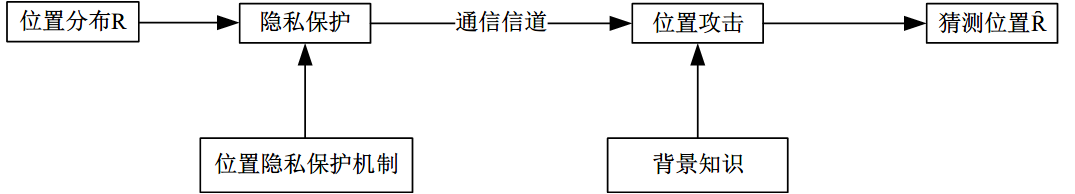
\includegraphics[width = 0.95\linewidth]{./figures/Communication-Model-for-Privacy-of-location.png}
	\caption{位置隐私保护场景通信模型}
	\label{fig:Communication-Model-for-Privacy-of-location}
\end{figure}

\subsection{相同背景知识下不同隐私保护机制的效果比较}\label{4.2}

在初始阶段,用户$u$处于一个真实区域$r_{i}$,则该用户处于区域$r_{i}$的概率为1,处于其它区域的概率为0,具体为

\begin{equation}
\begin{pmatrix}
R\\ 
P(R)
\end{pmatrix}=\begin{pmatrix}
r_{1} & r_{2} & \cdots  & r_{i} & \cdots  & r_{M}\\ 
0 & 0 & \cdots  & 1 & \cdots  & 0
\end{pmatrix}
\end{equation}

此时,隐私信源熵即位置分布$R$的熵为$H(R)=-\sum_{i=1}^{M}p(r_{i})\log p(r_{i})=0$。

\textbf{(1) 弱隐私保护强度的隐私度量}

当系统采用的位置隐私保护机制是位置泛化时,我们取用户$u$的发布位置从区域$r_{i}$泛化到$\left \{ r_{i-1},r_{i},r_{i+1},r_{i+2} \right \}$,可得到可观察位置分布的概率模型如下:
\begin{equation}
\begin{pmatrix}
{R}'\\ 
P({R}')
\end{pmatrix}=\begin{pmatrix}
{r}'_{1} & \cdots  & {r}'_{i-1} & {r}'_{i} & {r}'_{i+1}  & {r}'_{i+2} & \cdots & {r}'_{{M}'} \\ 
0 & \cdots & \frac{1}{4} & \frac{1}{4} & \frac{1}{4}  & \frac{1}{4} & \cdots & 0
\end{pmatrix}
\end{equation}

我们可以用$H({R}')=-\sum_{i=1}^{{M}'}p({r}'_{i})\log p({r}'_{i})=2$表示可观察位置分布的熵,等同于含敌手攻击的隐私保护信息熵模型下的熵$H(X/Y)$。

攻击者在获取到可观察位置分布后,结合其所拥有的背景知识进行分析,在一定的背景知识下,分析得到对用户$u$的推断位置分布的概率模型如下:

\begin{equation}
\begin{pmatrix}
\hat{R}\\ 
P(\hat{R})
\end{pmatrix}=\begin{pmatrix}
\hat{r}_{1} & \cdots  & \hat{r}_{i-1} & \hat{r}_{i} & \hat{r}_{i+1}  & \hat{r}_{i+2} & \cdots & \hat{r}_{\hat{M}} \\ 
0 & \cdots & \frac{1}{4} & \frac{1}{2} & \frac{1}{8}  & \frac{1}{8} & \cdots & 0
\end{pmatrix}
\end{equation}

此时我们可得$H(\hat{R})=-\sum_{i=1}^{\hat{M}}p(\hat{r}_{i})\log p(\hat{r}_{i})=1.75
$表示攻击者在具有背景知识的条件下对用户所在位置的不确定度的度量,等同于敌手攻击的隐私保护信息熵模型下的熵$H(X/YZ)$。

\textbf{(2) 强隐私保护强度的隐私度量}

当我们取泛化位置区域变大时,即隐私保护手段变强后,我们取用户$u$的发布位置从区域$\left \{ r_{i-1},r_{i},r_{i+1},r_{i+2} \right \}$变到$\left \{ r_{i},r_{i+1},\cdots,r_{i+7} \right \}$,可观察位置分布的概率模型为
\begin{equation}
\begin{pmatrix}
{R}'\\ 
P({R}')
\end{pmatrix}=\begin{pmatrix}
{r}'_{1} & \cdots & {r}'_{i}  & \cdots & {r}'_{i+7} & \cdots & {r}'_{{M}'}\\ 
0 & \cdots  & \frac{1}{8} & \cdots  & \frac{1}{8} & \cdots  & 0
\end{pmatrix}
\end{equation}

得到$H({R}')=-\sum_{i=1}^{{M}'}p({r}'_{i})\log p({r}'_{i})=3$表示可观察位置分布的熵,攻击者在相同的背景知识下,分析得到对用户$u$的推断位置分布的概率模型为
\begin{equation}
\begin{pmatrix}
\hat{R}\\ 
P(\hat{R})
\end{pmatrix}=\left( \begin{array}{cccccccccccc} 
\hat{r}_{1} & \cdots  & \hat{r}_{i} & \hat{r}_{i+1} & \hat{r}_{i+2} & \hat{r}_{i+3} & \hat{r}_{i+4} & \hat{r}_{i+5} & \hat{r}_{i+6} & \hat{r}_{i+7} & \cdots  & \hat{r}_{\hat{M}} \\
0 & \cdots  & \frac{1}{2} & \frac{1}{8} & \frac{1}{8} & \frac{1}{16} & \frac{1}{16} & \frac{1}{16} & \frac{1}{32} & \frac{1}{32} & \cdots  & 0\\
\end{array} \right)
\end{equation}

此时可得$H(\hat{R})=-\sum_{i=1}^{\hat{M}}p(\hat{r}_{i})\log p(\hat{r}_{i})=2.3125$表示攻击者在具有背景知识的条件下对用户所在位置的不确定度的度量,等同于敌手攻击的隐私保护信息熵模型下的熵$H(X/YZ)$。

由$2.3125>1.75$可验证含敌手攻击的隐私保护信息熵模型下~$H_{P_{i},A_{r}}(X/YZ)<H_{P_{j},A_{r}}(X/YZ)$~成立。

\subsection{相同隐私保护机制下不同隐私攻击的效果比较}

\textbf{(1) 弱隐私攻击强度的隐私度量}

同\ref{4.2}节弱隐私保护强度的隐私度量。

\textbf{(2) 强隐私攻击强度的隐私度量}

隐私保护机制同\ref{4.2}节弱隐私保护强度的隐私度量,攻击者在获取到可观察位置分布后,结合其所拥有的背景知识进行分析,在强隐私攻击强度下,分析得到对用户$u$的更准确的推断位置分布的概率模型如下
\begin{equation}
\begin{pmatrix}
\hat{R}\\ 
P(\hat{R})
\end{pmatrix}=\begin{pmatrix}
\hat{r}_{1} & \cdots & \hat{r}_{i-1}  & \hat{r}_{i} & \hat{r}_{i+1} & \hat{r}_{i+2} & \cdots  & \hat{r}_{{M}'}\\ 
0 & \cdots  & \frac{1}{6} & \frac{2}{3} & \frac{1}{12} & \frac{1}{12} & \cdots  & 0
\end{pmatrix}
\end{equation}

此时我们可得$H(\hat{R})=-\sum_{i=1}^{\hat{M}}p(\hat{r}_{i})\log p(\hat{r}_{i})=1.418$表示攻击者在具有背景知识的条件下对用户所在位置的不确定度的度量,等同于敌手攻击的隐私保护信息熵模型下的熵$H(X/YZ)$。

由$1.418<1.75$可验证含敌手攻击的隐私保护信息熵模型下~$H_{P_{i},A_{r}}(X/YZ)<H_{P_{i},A_{q}}(X/YZ)$~成立。

\section{小结}\label{sconclusion}

本章基于Shannon信息论提出了几种隐私保护信息熵模型,其关键出发点是将隐私保护系统视为一种通信模型,通过定义信源、信宿和信道、引入信息熵、平均互信息量、条件熵及条件互信息等概念,初步给出了不同场合的隐私信息度量、隐私泄露度量、隐私保护强度量化和攻击能力量化等方法,并且初步考虑了含隐私信息主观感受的信息熵模型。本章的工作虽然只给出了较为基本的信息熵模型,但为解决隐私保护系统的量化问题建立了一个可行的体系基础,相信在信息论相关成果的支撑下,其相关研究可以不断深入,包括连续隐私信源的研究、更复杂的多隐私信源模型、基于随机过程的信息熵模型、贝叶斯隐私信息熵模型和马尔柯夫隐私信息熵模型等,都具备了深入研究的可行性。












